\section{Research Project Proposal} \label{research-proposal-section}
\subsection{Motivation}
The studies evaluated in the previous section applied traditional ways of measuring investor sentiment. In the following we explain why and how modern measurements add value to investor sentiment research, and illustrate how we will apply them in our own research.
\par
Traditional investor sentiment measures such as AAII or II have provided direct insights on investor sentiment for multiple decades and most of the studies have employed these measures to investigate the connection between investor sentiment and stock returns. Furthermore, indirect sentiment measures, such as VIX, consumer confidence, market performance or a weighted measure proposed by Baker and Wurgler (2007), which combines multiple indirect proxies, have been used to better understand the relationship. With the rise of technology and the internet, new ways to measure investor sentiment have emerged which are utilized by traders all over the world. Those new measures capture investor sentiment in two distinct ways. First, a new way to measure investor sentiment on a large scale appeared with the rise of the platform StockTwits, which is a social media platform specifically geared towards stock traders. Users exchange thoughts on stocks and indices by posting messages and engaging in conversations. Hereby, they can specifically label their posts as bearish or bullish and thus directly share their sentiment. With 7 million monthly active users, StockTwits contains a large array of sentiment data and this sentiment is likely to have an impact on the decision making process of the individual investor. Collecting and organizing this data allows an entirely new, big-data based approach to measuring investor sentiment - similar to the surveys employed by organizations such as AAII or II on a large scale. The advantage of these new big data approaches over traditional methods is that for the first-time, sentiment towards specific stocks or indices can be related to the returns of that specific stock or index. The amount of data enables researchers to analyse sentiment and returns on a daily basis, not only weekly or monthly. Moreover, it is now possible to analyse whether the so-called "wisdom of the crowds" adds value to the stock market and to financial industry.
\par
The second approach to measuring sentiment is through intelligent algorithms which scan social media platforms for stock-related posts and employ Natural Language Processing (NLP) algorithms to categorize these tweets as bullish or bearish. The goal of successful NLP is to train computers to correctly process natural language and categorize text as a human brain would. Prior research on investor sentiment on Twitter and subsequent stock returns was conducted by Bollen et al. (2011), Rao et al. (2012), Chen et al. (2013) and Skuza et al. (2015). These authors developed own algorithms which classify whether the tweet about a certain stock is bullish, bearish or neutral. With computing power becoming cheaper and more readily available, organizations developed own NLP algorithms and are using them on large scale. PsychSignal is such an organization; their algorithms evaluate both the Twitter and the StockTwits feeds and translate each post into bullish or bearish sentiment. The characteristics of posts are then aggregated by the related symbol and day. PsychSignal offers all their data to the public for free on Quantopian, a platform where researchers can use this investor sentiment measure to experiment new connections between stock returns and investor sentiment. This data is also used by professional, quantitative investors to develop and improve their trading algorithms.
\par
The goal of our research is to evaluate these modern investor sentiment measures, which are used by the public and influence investment decisions. Our research approach is on three levels: (1) compare these new sentiment measures to more traditional measures like AAII (2) compare the PsychSignal NLP algorithm to the direct sentiment measure from StockTwits users and (3) investigate the relationship between the modern investor sentiment measures and stock returns, which is the main hypothesis of our research. 

\subsection{Research Strategy} \label{research_strategy}
For the first and second level of our research, we will apply time series studies, focusing on correlation analyses. There are three modern sentiment measures (databases) available to us which will be used in this research: (1) StockTwits (direct sentiment measure from StockTwits users), (2) PS:StockTwits (StockTwits messages analysed by the PsychSignal NLP algorithm) and (3) PS:Aggregated (aggregated Twitter and StockTwits messages analysed by the PsychSignal NLP algorithm). Since data mining and text sentiment analysis are two modern and new concepts, we are interested in investigating the extent to which the results of the modern way of capturing investor sentiment through social media and tweets overlaps with the traditional sources of investor sentiment employed in existing studies. Furthermore, we decided to investigate the relationship between different modern sentiment measures since they differ in the way data is collected. The correlation analysis is a viable tool in this situation since our interest is in correlation/association and not causation. A high correlation between the measures shows that the sentiment measures follow a similar pattern, whereas low correlation implies that the sentiment measures differ. This test will not imply causation.
\par
The research strategy for the third level of our research points to the main hypothesis effect of investor sentiment on subsequent stock returns. For this specific research question, the perfect strategy would be an experimental study. Experiments are the most powerful tool in proving direct causation since only the independent variable is manipulated, while other variables and factors are kept constant. On the one hand, this results in high internal validity of the strategy, ensuring we have found a direct effect of the independent variable on the dependent one. On the other hand, an experimental study applied to investor sentiment and stock returns comes with many barriers which cannot be overcome.
\par
There are two main problems with an experiment. Firstly, the limited time frame of this study makes it impossible to conduct an experiment which has generalizable results. The analysis of investor sentiment over stock returns should be conducted over a longer period so that a general trend can be observed, and not just temporary positive or negative trends. Since the time frame of our research has a timespan of few months, this period is not sufficient to draw precise conclusions. Secondly, an experiment suggests that the experimental groups should not be influenced by any external factors. Regarding investor sentiment, this implies that investors cannot be allowed to access information other than what is provided by the researchers. In this case, participants must be controlled and finding willing people to be part of this study might not be easily achieved.
\par
With experiments not being a feasible option, the research strategy which fits our purposes is the panel study. Although it presents lower internal validity for causal claims, it solves many of the dilemmas posed by the experiment, and, furthermore, it has a higher level of ecological validity: the findings can be generalised to the real-life since the researcher has little to no influence. The panel study is suitable in this case because we want to study how changes in the independent variable affect the dependent variable over time. Moreover, having two continuous variables and studying only two stocks (as explained in the next section), it is possible to employ a time series study, where the panel is made of the data points at a certain moment in time for only one focal unit. This time series study allows the use of time lags between variables. Our point of interest is the regression coefficient which is discussed in section \ref{effect size parameter} in more detail.

\subsection{Population} \label{population}
Regarding the population of interest, we plan to investigate the effect of investor sentiment on S\&P 500 and Dow Jones Industrial Average (DJIA) stocks. DJIA stocks are large, traditional American firms, whereas S\&P 500 has a wider breadth of companies from different industries, with different market capitalisation and volatility. Since there is not sufficient investor sentiment data for each individual stocks from S\&P 500 and DJIA, we decided to work with indices and not at an individual stock-level. Indices are useful in measuring the value of a given section of the market, and they also provide a reliable proxy for the performance of the containing stocks (Fisher and Statman 2000, Brown and Cliff 2006). Considering the availability of sentiment data in our data sources, the final decision was to use exchange-traded funds (ETFs) which specifically track S\&P 500 and DIJA. These index funds seek to replicate the performances of their respective indices. Hence, for S\&P 500 we use the S\&P 500 Index ETF, denoted \$SPY, and for the Dow Jones Industrial Average we employ the DJIA ETF, referred to as \$DIA.

\subsection{Time Frame} \label{timeframe}
The current literature varies in terms of time frame, aggregation of data and time lags. Because our research employs modern approaches of investor sentiment measures, these characteristics are mainly determined by the practical side of the research. The available data from StockTwits starts in 2010; however, since the platform's popularity grew over the years, the data from the first years is insufficient to draw conclusions for the overall investor sentiment regarding a certain stock or ETF. Similarly, PsychSignal provides different datasets which start in between 2009 and 2010 and also contain small numbers of analysed messages for the first years. Furthermore, the data we received was daily and many data points did not provide a reliable measure of investor sentiment for that day because of a lack of posts.
\par
Considering the above-mentioned reasons, we have aggregated the daily data regarding symbols \$SPY and \$DIA on weekly and monthly basis. Then, in order to decide on a time frame for our analysis, we have computed the means of these aggregated values to observe how the average number of weekly and monthly analysed posts have changed over the years. Figures~\ref{fig:msg_spy_agg} and~\ref{fig:msg_dia_agg} below present these values for sentiment data from the dataset PS:Aggregated over the period 2012-2016.

\begin{figure}[ht]
\centering
\caption{\label{fig:msg_spy_agg}Analysed posts by NLP algorithm for symbol \$SPY}
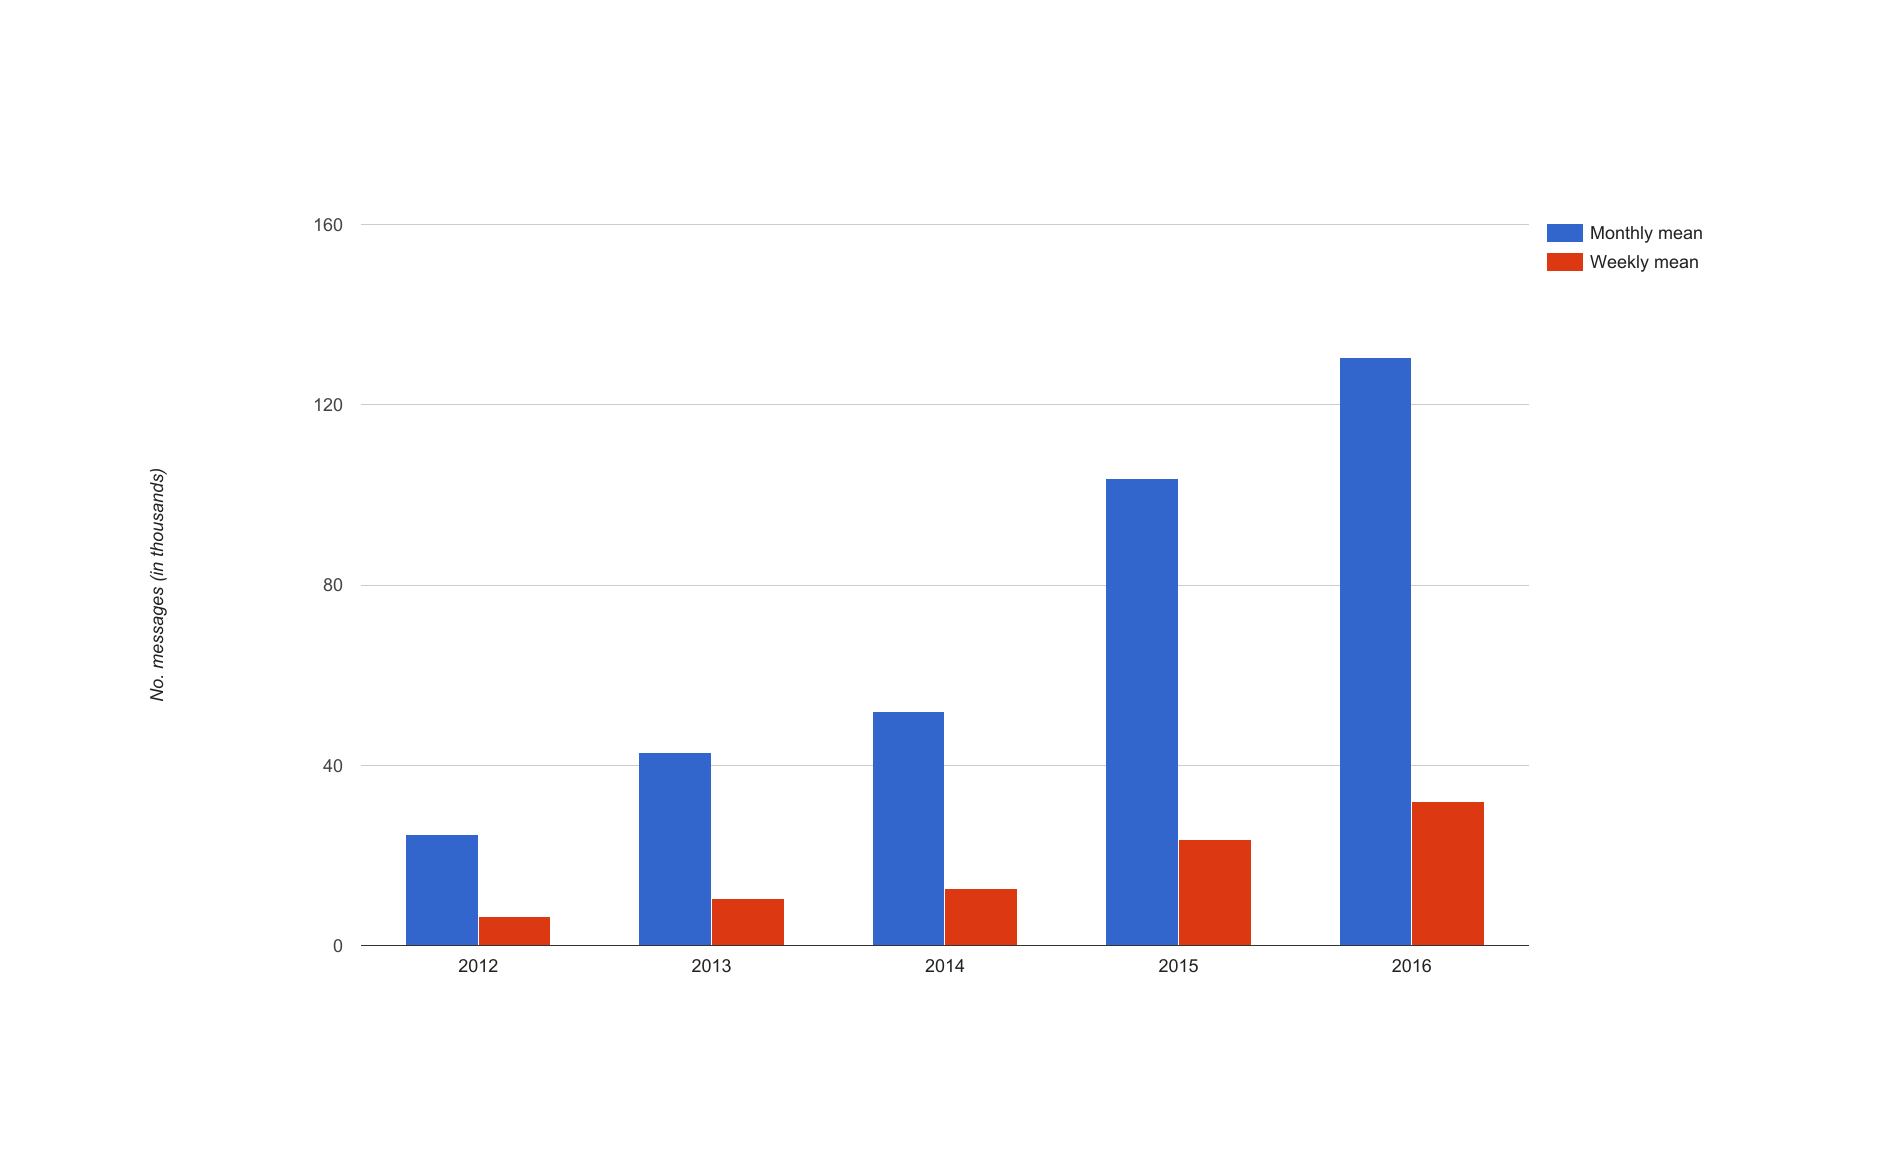
\includegraphics[width=0.8\textwidth]{figures/msg_spy_agg.png}
\end{figure}

\begin{figure}[ht]
\centering
\caption{\label{fig:msg_dia_agg}Analysed posts by NLP algorithm for symbol \$DIA}
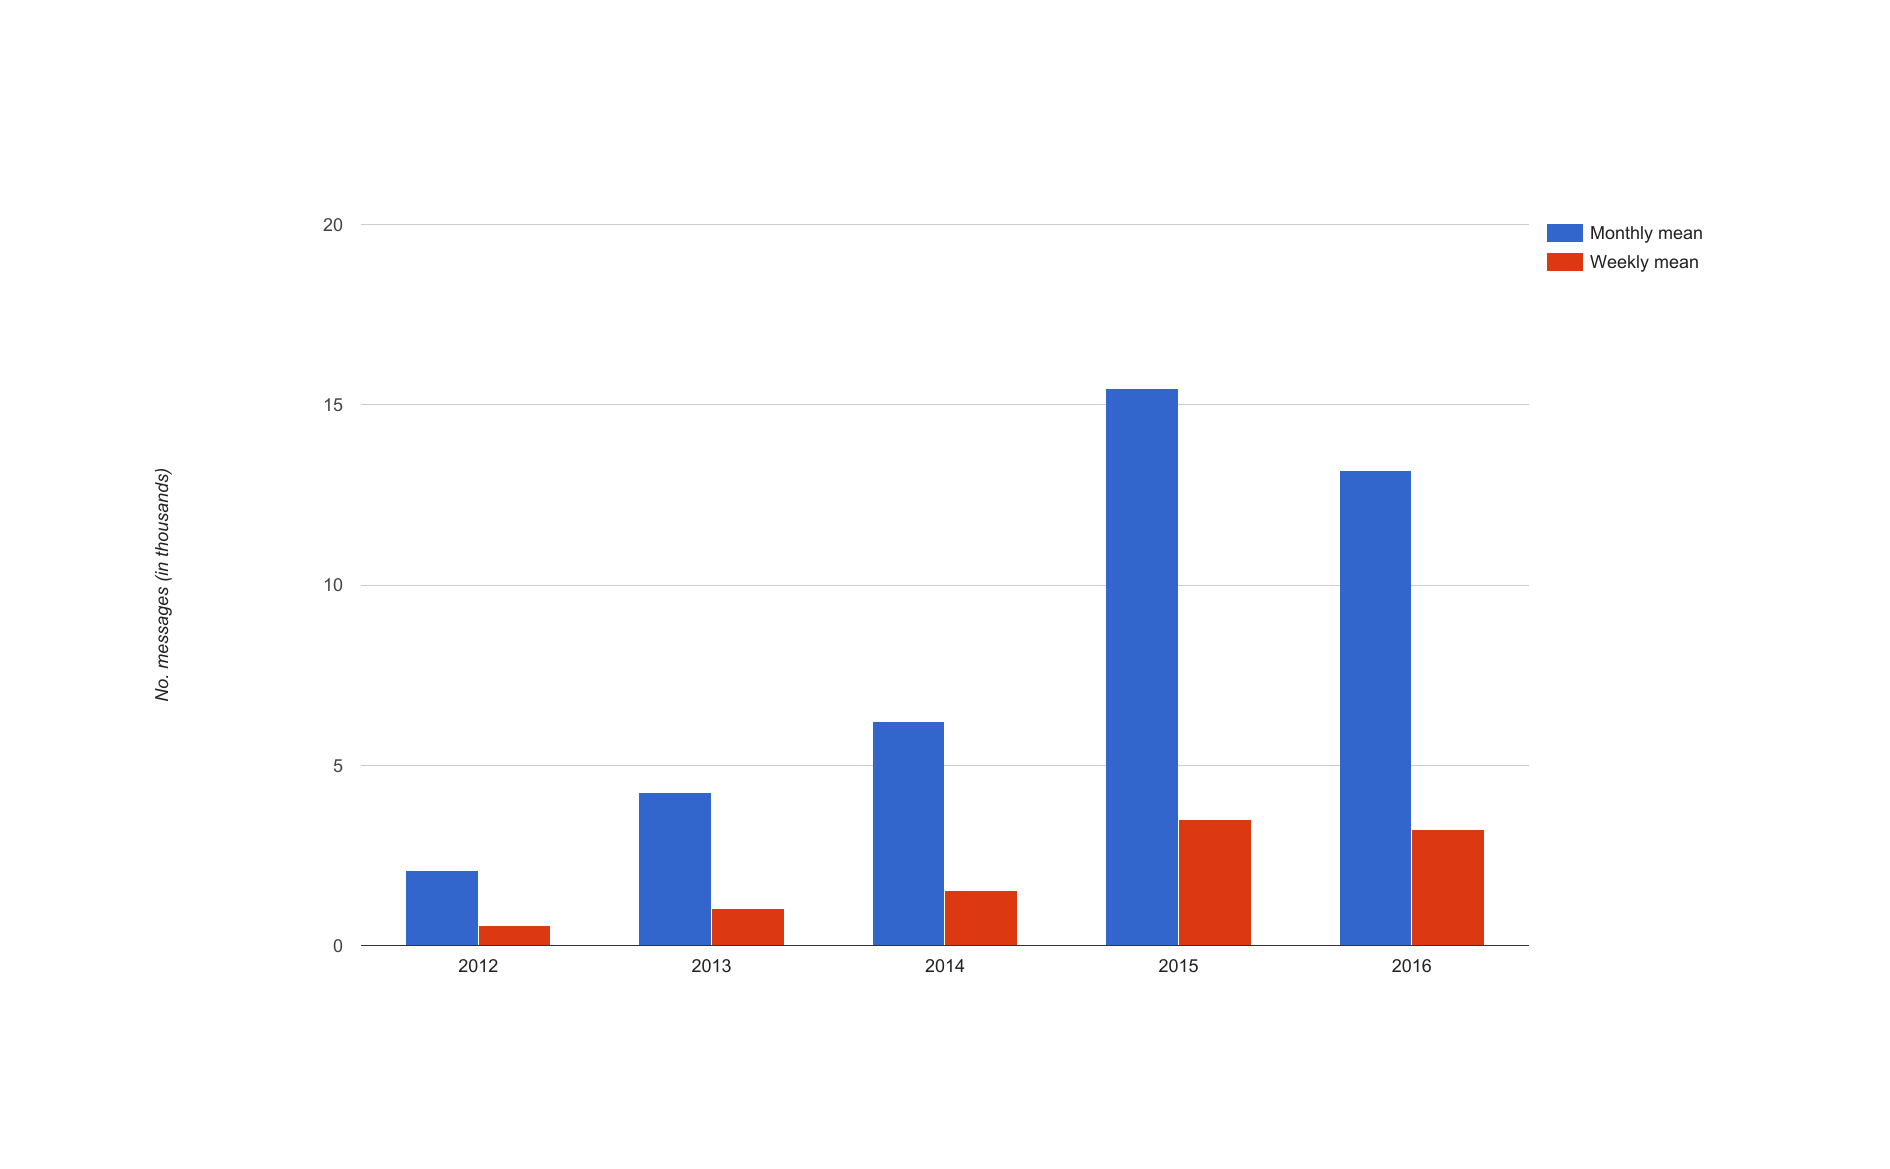
\includegraphics[width=0.8\textwidth]{figures/msg_dia_agg.png}
\end{figure}

The figures show a large difference between the years of interest. The monthly mean of \$SPY related posts increased from 24,531 in 2012 to 130,531 in 2016, while \$DIA related posts started at 2,094 in 2012 and reached 13,167 in 2016. The weekly means show similar trends, reaching five times the initial values. Based on these results, we have decided to work with data from 01/01/2014 until 31/12/2016, covering three full years.
\par
Regarding the time lags studied, we chose to pursue multiple time lags in order to investigate the effect of sentiment both on short-term and long-term returns. Hence, we choose weekly lags of 1, 4, 6, 8 and 12 weeks, and monthly lags of 1, 2 and 3 months.

\subsection{Data Matrix}
The choice of research strategy has a high impact on the data matrix and its structure. Since our research is time-series study (a type of panel study), the data matrix needs to present the changes in variables over time. The rows of the matrix represent different cases, and the columns are the characteristics of the case. Since the characteristics of the tests to be performed vary widely, we present a sample of the data matrix in Table~\ref{tab:data-matrix} below. This data matrix presents the ETF \$SPY, weekly aggregated data with 6-weeks lag, change in investor sentiment as independent variable and stock returns as dependent variable:

\begin{table}[ht]
\centering
\begin{tabular}{ c c c c }
Case (Stock: SPY) & Week & Change in investor sentiment & Stock return  \\\hline
SPY & 1 & \( \Delta sent_1 \) & \( return_7 \) \\
SPY & 2 & \( \Delta sent_2 \) & \( return_8 \) \\
SPY & 3 & \( \Delta sent_3 \) & \( return_9 \) \\
... & ... & \( ... \) & \( ... \) \\
SPY & 151 & \( \Delta sent_{151} \) & \( return_{157} \) \\
\end{tabular}
\caption{\label{tab:data-matrix}Example Data Matrix}
\end{table}

All the variations presented in sections~\ref{research_strategy},~\ref{population} and~\ref{timeframe} lead to 96 regression analyses which are different regarding the studied ETF, type of data aggregation, dataset, time lag and type of independent variable (absolute level of sentiment or change in level of sentiment). The regressions follow the formula below, where $\alpha$ is the intercept and $\beta$ is the regression coefficient:
\begin{equation}
Return_{t+lag} = \alpha + \beta * sentiment_t
\end{equation}

Plotting an exemplary time-series regression for \$SPY sentiment change, weekly aggregated, and returns six weeks later results in the graph presented in figure~\ref{fig:figure1}.

\begin{figure}
\centering
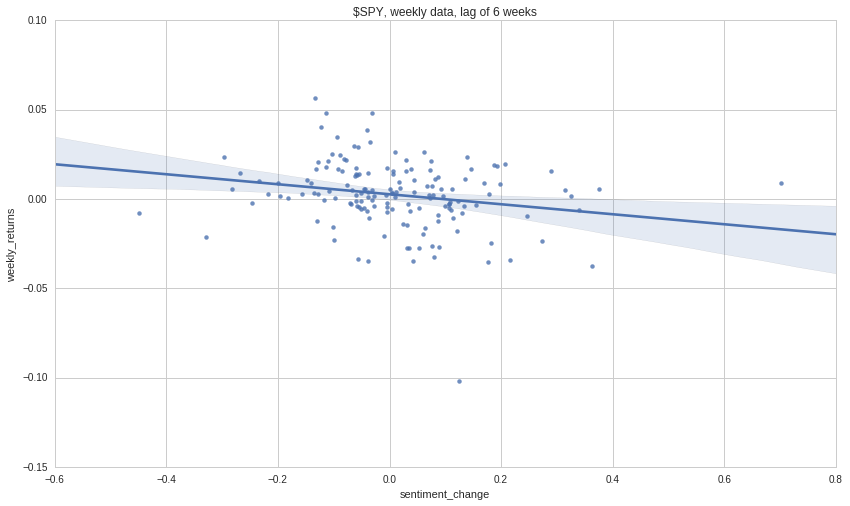
\includegraphics[width=1\textwidth]{figures/figure1.png}
\caption{\label{fig:figure1}Scatter Plot and Regression line}
\end{figure}

\newpage

\subsection{Measurement Protocol}
Although StockTwits and PsychSignal work with different algorithms and provide different ways to measure investor sentiment, the collection and manipulation of data leads to similar datasets. Data from StockTwits contains information about each post and the user who posted it, as well as data about the related stock; included in this is the indication whether the post is bullish, bearish or neutral. After storing this data in a database, we can filter it on the stocks of interest and make weekly or monthly aggregates on the number of bull and bear messages. The sentiment level is then determined as the percentage of bullish messages from the total of bullish and bearish messages:
\begin{equation}
BullPerc = Bull_{messages} / (Bull_{messages} + Bear_{messages})
\end{equation}
To compute the change in sentiment level in period t+1, we use the following formula:
\begin{equation}
Sent_{change} = (BullPerc_{t+1} - BullPerc_t ) / BullPerc_t
\end{equation}
For PsychSignal data, the total number of bullish and bearish messages is already aggregated daily, and thus we can use these totals. After filtering the data on stock and date, we sum up the numbers on weeks or months, according to our time-frame. The percentage of bullish messages per period and the change in it are computed using the same formulas as above.

\subsection{Specification of the Effect Size Parameter} \label{effect size parameter}
After establishing the cases in the above data matrix using the data from StockTwits, PsychSignal and stock return data, we will quantify the strength of the relationship by establishing an effect size. For the comparison of different measures of investor sentiment, the correlation coefficient is used. With this coefficient, we measure whether there is linear relationship between two variables and the strength and direction of this relationship. The coefficient of correlation takes values between -1 and 1, where r=1 shows a very strong positive relationship. 
\par
To measure the magnitude of the relationship between investor sentiment and stock returns, we use regression coefficients. We test with both the change and the absolute value of investor sentiment as independent variable. When change in sentiment is used, the effect size denotes the magnitude of the stock return change influenced by the change in investor sentiment. When using absolute values, we investigate what is the magnitude of the influence of level of sentiment on stock returns.